\documentclass{article}

\usepackage[fleqn]{amsmath}
\usepackage{fontspec}
\usepackage{xcolor}
\usepackage{tikz}
\usepackage{ragged2e}
\usepackage{graphicx}
\usepackage{pgfplots}
\pgfplotsset{width=10cm, compat=1.5}

\usetikzlibrary{angles, quotes}
\setmainfont{DejaVu Sans}



\begin{document}

{\fontsize{20}{18} \selectfont Домашнее задание 5}
\newline




{\fontsize{14}{10} \selectfont  Построить графики функций (ниже дан пример как это делать): } \newline



{\fontsize{12}{8} \selectfont \color{gray} Графики вида: $y(x) = k\cdot x + b $ являются прямой на координатной плоскости.
Любую прямую можно построить по двум точкам, значит нужно найти две точки графика. 
В примере ниже построен график функции $y(x) = 3\cdot x + 1$ по двум точкам: (0,1); (1,4) они выделены красным цветом на графике. 
Координату $x$ в этих точках выбираешь сам, 
$y$ получаешь подстановкой $x$ в функцию: $y(0) = 3\cdot 0 + 1 = 1; \; \; y(1) = 3\cdot 1 + 1 = 4$, 
по этим двум точкам можно построить прямую, которая и будет графиком функции $y(x) = 3\cdot x + 1$} \\ \\

\vspace{2cm}

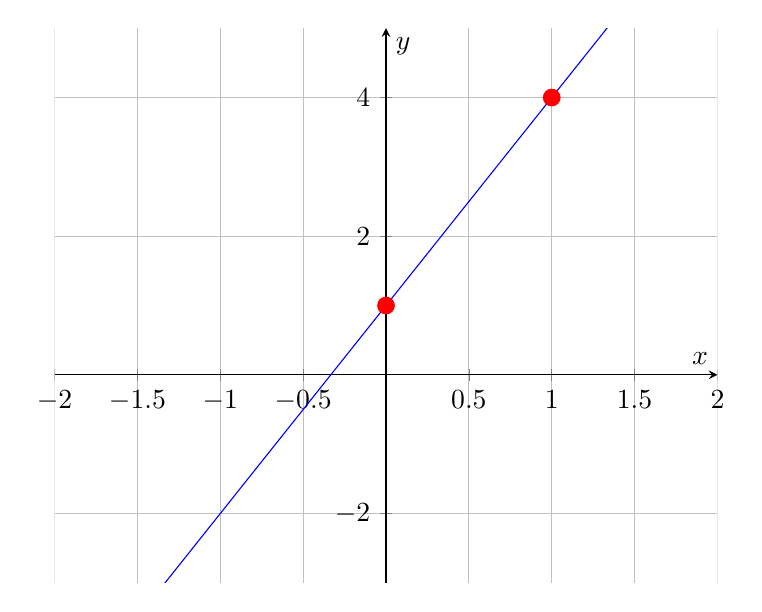
\begin{tikzpicture}
    \begin{axis}[
        axis lines = middle, % Оси в центре
        xlabel = \( x \),   % Подпись оси X
        ylabel = \( y \),   % Подпись оси Y
        xmin = -2, xmax = 2, % Пределы по X
        ymin = -3, ymax = 5,  % Пределы по Y
        grid = both
    ]
        \addplot[domain=-3:3, samples=100, color=blue] {3*x + 1}; % График функции

        \addplot[only marks, mark=*, mark size=3pt, color=red] coordinates {
            (0, 1)
            (1, 4)
        };

    \end{axis}
\end{tikzpicture}

\vspace{4cm}

{\fontsize{13}{9} \selectfont Задания на построение графика} \newline




1. $y(x) = 2\cdot x + 3$ \\



2. $y(x) = 4\cdot x - 2$ \\



3. $y(x) = 12\cdot x - 8$ \\



4. $y(x) = x$ \\



5. $y(x) = 4$


\end{document}